%!TEX program = xelatex
\documentclass[aspectratio=169]{ctexbeamer}
% \usepackage{physics}
                        %%% 宽高比说明 %%%%
%% ctexbeamer宏包支持各种宽高比，但本模板只适配了4:3（默认）和16:9的宽高比背景。
%% 添加选项aspectratio=169或aspectratio=43可以更改宽高比，默认是4:3
\usepackage[bluetheme]{ustcbeamer}
\input{ustctheme.tex}
                        %%% ustcbeamer说明 %%%%
%% 宏包使用了TikZ代码形式的背景文件（在子文件夹theme中），默认选项"bluetheme"，是科大校徽的蓝色；
%% 此外ustcbeamer还内置了红色和黑色主题"redtheme","blacktheme"。

                        %%% 自定义你的主题颜色 %%%
%% 一旦使用了下述命令就会覆盖ustcbeamer的内置颜色选项，你可以设置自己喜欢的RGB色值：
% \definecolor{themecolor}{RGB}{0,150,0}
% \definecolor{themecolor}{RGB}{0,150,150}
% \definecolor{themecolor}{rgb}{0,0.5,0.3}
%%%%%%%%%%%%%%%%%%%%%%%%%%%%%%%%%%%%%%%%%%%%%%%%%%%%%%%%%%%%%%%%%%%%%%

\usepackage{graphicx}
\usepackage{booktabs}
\usepackage{tabularx}
\usepackage{array}
\usepackage{ragged2e}
\usepackage{adjustbox}
\graphicspath{{figures/}}

\newcolumntype{Y}{>{\RaggedRight\arraybackslash}X}
\newcommand{\code}[1]{\texttt{#1}}
\newcommand{\diagramfig}[2]{%
  \begin{center}
  \IfFileExists{#1}{%
    \includegraphics[width=\textwidth,height=0.68\textheight,keepaspectratio]{#1}%
  }{%
    \fbox{\begin{minipage}[c][0.42\textheight][c]{0.86\textwidth}
      \centering
      \large 请放置图文件\\[0.6em]
      \texttt{#1}\\[0.6em]
      \small #2
    \end{minipage}}%
  }
  \end{center}
}

\title[Agent Runtime]{
    Agent Runtime 项目期末汇报
}
\author[张贺淇]{报告人：张贺淇\quad 陈雨桥}
\institute[USTC]{
中国科学技术大学
}
\date{2026 年 7 月 2 日}

\begin{document}

%--------------------
%标题页
%--------------------
\maketitleframe

%--------------------
%目录页
%--------------------
\begin{frame}%
    \frametitle{大纲}%
    \tableofcontents[hideallsubsections]%
\end{frame}%

%--------------------
%节目录页
%--------------------
\AtBeginSection[]{
\setbeamertemplate{footline}[footlineoff]
  \begin{frame}%
    \frametitle{大纲}
    \tableofcontents[currentsection,subsectionstyle=show/show/hide]
  \end{frame}
\setbeamertemplate{footline}[footlineon]
}

%--------------------
%子节目录页
%--------------------
\AtBeginSubsection[]{
\setbeamertemplate{footline}[footlineoff]
  \begin{frame}%
    \frametitle{大纲}
    \tableofcontents[currentsection,subsectionstyle=show/shaded/hide]
  \end{frame}
\setbeamertemplate{footline}[footlineon]
}

\section{项目背景与定位}

\begin{frame}
  \frametitle{项目定位与整体构成}
  本项目面向 Android 端侧智能体，构建一套可本地部署、可结构化执行、可观测且可扩展的 Agent Runtime。

  \vspace{0.5em}
  项目主体由两条平级技术线协同组成：
  \begin{itemize}
    \item 端侧 LLM 推理框架：负责 Android 本地模型加载、推理、KV Cache、量化、GPU/Vulkan 优化，并提供兼容 OpenAI 的模型服务接口。
    \item Action Fabric 结构化执行系统：负责把模型生成的任务计划表示为 Action DAG，并完成校验、调度、执行、恢复和审计，同时把结构化 Action 映射到 Android SDK、系统服务、ContentResolver、Intent 和权限协调组件。
  \end{itemize}

  \vspace{0.5em}
  整体协作关系是：本地模型负责规划与生成，Action Fabric 负责可靠执行，并将任务落到具体 Android 系统能力上。
\end{frame}

\begin{frame}
  \frametitle{移动端 Agent 的真实瓶颈}
  移动端 Agent 的瓶颈不只是模型参数规模，还包括：
  \begin{itemize}
    \item 本地推理延迟高，弱网络或离线场景不能依赖云端补偿。
    \item 多轮模型调用会放大端到端等待时间。
    \item 上下文窗口有限，工具结果反复进入 prompt 会快速膨胀。
    \item 手机内存、功耗、温控和后台执行限制更严格。
    \item Android 系统能力涉及权限、Intent、前台服务和用户确认。
  \end{itemize}

  \vspace{0.5em}
  因此，端侧 Agent 需要的是一个可靠的执行系统，而不只是一个会调用工具的模型。
\end{frame}

\begin{frame}
  \frametitle{传统 Agent Loop 的问题}
  \begin{columns}[T,onlytextwidth]
    \begin{column}{0.58\textwidth}
      % Mermaid 导出图：传统 Agent Loop 时序图
      \diagramfig{figures/agent-loop-problem.pdf}{对应 Markdown 中“传统 Agent Loop 的问题”的 sequenceDiagram。}
    \end{column}
    \begin{column}{0.39\textwidth}
      \small
      传统做法把执行路径藏在自然语言上下文里。

      \vspace{0.5em}
      \begin{block}{主要问题}
        \scriptsize
        \begin{itemize}
          \item 每一步成功后仍要回到模型判断下一步。
          \item 独立工具调用也容易被串行化。
          \item 执行历史以文本形式堆叠，不利于校验、调试、回放和审计。
          \item 失败恢复依赖模型临场判断，容易重复副作用。
        \end{itemize}
      \end{block}
    \end{column}
  \end{columns}
\end{frame}

\begin{frame}
  \frametitle{从推理驱动到调度驱动}
  对于移动端 Agent，执行链路应该从“推理驱动”转向“调度驱动”。

  \vspace{0.5em}
  模型输出一次结构化计划，Runtime 显式维护依赖关系和状态；成功路径不反复唤醒模型，只有格式错误、节点失败、权限确认或异常恢复时才回退给模型。

  \vspace{0.5em}
  \scriptsize
  \begin{tabularx}{\textwidth}{p{0.18\textwidth}Y}
    \toprule
    目标 & 含义 \\
    \midrule
    可校验 & 执行前发现缺参、错参、未知工具、循环依赖 \\
    可调度 & Runtime 根据 DAG 自动计算 ready set \\
    可并行 & 互不依赖的节点可以批量异步执行 \\
    可恢复 & 失败后按副作用等级、重试预算和诊断信息处理 \\
    可审计 & 节点状态迁移、输出和诊断可记录、可回放 \\
    \bottomrule
  \end{tabularx}
\end{frame}

\begin{frame}
  \frametitle{业界如何缓解 Agent Loop 瓶颈}
  围绕多轮推理、上下文膨胀、隐式依赖和并行不足，业界方案正在从“让模型看到更多”转向“让模型每轮只看到最有用、最可信、最短的信息”，并把执行过程结构化。

  \vspace{0.3em}
  \tiny
  \begin{tabularx}{\textwidth}{p{0.21\textwidth}Y Y}
    \toprule
    业界方向 & 关键做法 & 设计启发 \\
    \midrule
    MCP / Tool Calling & 标准化工具名称、schema、资源链接和工具元数据，让模型能可靠连接外部能力 & 工具需要清晰边界：模型负责选择能力，系统负责约束能力 \\
    Context engineering / management & write / select / compress / isolate；工具结果引用化；tool retrieval；热/温/冷上下文分层 & 上下文需要被管理：不是塞入全部历史，而是按需提供短、可信的信息 \\
    Workflow patterns & Anthropic 将 prompt chaining、routing、parallelization、orchestrator-workers 等归为 workflow 类模式 & 确定性执行路径适合沉淀为 Workflow，模型负责规划和处理开放问题 \\
    Structured Graph & arXiv 2604.11378 将 Agent Loop 视为 single-ready-unit scheduler，并提出把控制流提升为静态 DAG & 执行过程需要显式化：依赖、并发、恢复不应只藏在自然语言历史中 \\
    \bottomrule
  \end{tabularx}

  \vspace{0.45em}
  \footnotesize
  业界正在把 Agent 从“长上下文里的连续对话”推进为“模型决策 + 结构化工具 + 可管理上下文 + Workflow 编排”的系统工程。

  \vspace{0.3em}
  \tiny
  参考：MCP Introduction；Anthropic, \emph{Building Effective Agents}；arXiv:2604.11378。
\end{frame}

\section{系统架构与技术路线}

\begin{frame}
  \frametitle{总体架构}
  % Mermaid 导出图：README 中“系统协作关系”的完整架构图
  \diagramfig{figures/system-architecture.pdf}{对应 Markdown 中“总体架构”的 flowchart TB。}
\end{frame}

\begin{frame}
  \frametitle{技术路线总览}
  % Mermaid 导出图：技术路线总览 flowchart LR
  \diagramfig{figures/technical-route.pdf}{对应 Markdown 中“技术路线总览”的 flowchart LR。}

  路线：Workflow YAML 表达计划，Rust Dispatcher 承担调度和恢复，Protocol Buffers + gRPC 打通跨语言执行链，Android Action Runtime 落地 Android 系统能力。
\end{frame}

\begin{frame}[fragile]
  \frametitle{Workflow YAML：结构化计划}
  \begin{columns}[T,onlytextwidth]
    \begin{column}{0.65\textwidth}
      \tiny
\begin{verbatim}
version: 1
id: device-report
steps:
  - id: device
    action: device_info
    inputs:
      includeHardware: true
  - id: network
    action: network_status
    inputs:
      includeDetails: true
  - id: power
    action: power_status
    inputs:
      includeDetails: true
  - id: final_report
    action: subagent
    inputs:
      prompt: "根据 ${device} ${network} ${power} 生成设备状态摘要。"
output: final_report
\end{verbatim}
    \end{column}
    \begin{column}{0.32\textwidth}
      \begin{block}{DAG 结构}
        \scriptsize
        \code{device}、\code{network}、\code{power} 互不依赖，可并发执行；\code{final\_report} 依赖三者。
      \end{block}

      \begin{block}{推理轮数与输出}
        \tiny
        主 Agent 控制链从约 4 轮（选三个工具 + 最终回答）降为 1 轮（生成完整计划）。成功后不再回主 Agent 临时总结；用户拿到的是首轮计划中 \code{output: final\_report} 指定的节点结果。
      \end{block}

      \begin{block}{缩减上下文}
        \tiny
        工具输出保存在 runtime state，下游通过 \code{\$\{device\}} 等引用结果，避免完整工具历史反复进入模型上下文。
      \end{block}
    \end{column}
  \end{columns}
\end{frame}

\begin{frame}
  \frametitle{Rust Dispatcher：从计划到执行}
  \begin{columns}[T,onlytextwidth]
    \begin{column}{0.58\textwidth}
      % Mermaid 导出图：Rust Dispatcher 执行流程
      \diagramfig{figures/dispatcher-execution.pdf}{对应 Markdown 中“Rust Dispatcher：从计划到执行”的 flowchart TD。}
    \end{column}
    \begin{column}{0.39\textwidth}
      \small
      Engine 不询问模型“下一步是什么”，而是根据 DAG 和节点状态推进执行。

      \vspace{0.5em}
      \begin{block}{调度职责}
        \scriptsize
        \begin{itemize}
          \item Loader 校验依赖、引用、缺参和循环。
          \item Dispatcher 维护节点状态并计算 ready set。
          \item 同一 ready set 内批量异步执行。
          \item 非幂等和高风险节点按策略受到串行约束。
        \end{itemize}
      \end{block}
    \end{column}
  \end{columns}
\end{frame}

\begin{frame}
  \frametitle{Rust-Kotlin 跨语言执行链}
  % Mermaid 导出图：Rust-Kotlin gRPC sequenceDiagram
  \diagramfig{figures/rust-kotlin-grpc-chain.pdf}{对应 Markdown 中“Rust-Kotlin 跨语言执行链”的 sequenceDiagram。}

  这条链路让 Rust 调度层和 Android 能力层解耦，后续扩展 Action 不需要重写调度器。
\end{frame}

\begin{frame}
  \frametitle{Android Action Runtime：封装 Android 能力}
  Android Action Runtime 已注册 59 个 Android Action：

  \vspace{0.4em}
  \scriptsize
  \begin{tabularx}{\textwidth}{p{0.22\textwidth}Y}
    \toprule
    能力类别 & 代表 Action \\
    \midrule
    设备与系统 & \code{device\_info}、\code{system\_info}、\code{power\_status}、\code{storage\_info} \\
    网络与连接 & \code{network\_status}、\code{http\_call}、\code{wifi\_toggle}、\code{bluetooth\_toggle} \\
    应用与 Intent & \code{list\_installed\_apps}、\code{launch\_app}、\code{intent\_show\_map}、\code{intent\_compose\_email} \\
    数据与文件 & \code{read\_file}、\code{search\_files}、\code{clipboard\_read}、\code{clipboard\_copy} \\
    个人信息 & \code{search\_contacts}、\code{read\_sms}、\code{list\_calendar\_events} \\
    媒体与传感 & \code{take\_photo}、\code{record\_audio}、\code{screenshot}、\code{screen\_record} \\
    \bottomrule
  \end{tabularx}

  \vspace{0.4em}
  \normalsize
  封装方式：每个能力实现为结构化 Action，定义输入数据类、输出数据类和 \code{execute} 逻辑；只读能力通过 Android SDK、系统服务或 ContentResolver 查询；应用交互能力通过标准 Intent 封装；相机、录音、截图、通知等能力由专门协调组件处理权限、生命周期和系统授权。
\end{frame}

\begin{frame}
  \frametitle{安全、权限与治理}
  策略不由模型自述，而由可信 registry metadata 注入：

  \vspace{0.4em}
  \scriptsize
  \begin{tabularx}{\textwidth}{p{0.22\textwidth}Y}
    \toprule
    治理维度 & 设计 \\
    \midrule
    风险等级 & \code{Low}、\code{Medium}、\code{High}、\code{Critical} \\
    副作用等级 & \code{Pure}、\code{Idempotent}、\code{NonIdempotent} \\
    用户确认 & 高风险节点进入 \code{WaitingHuman} \\
    重试预算 & 按 action metadata 控制，非幂等失败不自动重试 \\
    超时控制 & 节点级超时，避免长时间阻塞 \\
    审计日志 & 记录节点状态迁移与诊断信息 \\
    \bottomrule
  \end{tabularx}

  \vspace{0.6em}
  \normalsize
  模型不能伪造 \code{policy}、\code{sideEffect}、\code{retryBudget}、\code{timeoutMs} 等策略字段。
\end{frame}

\begin{frame}
  \frametitle{恢复机制：失败后的受控修正}
  \small
  恢复机制的目标不是“失败后让模型重新猜一遍”，而是尽可能保留已完成的确定性执行，并把可修正的信息压缩反馈。

  \vspace{0.4em}
  \scriptsize
  \begin{tabularx}{\textwidth}{p{0.22\textwidth}Y}
    \toprule
    情况 & Runtime 行为 \\
    \midrule
    纯节点失败 & 在重试预算内自动重试 \\
    幂等节点失败 & 可按策略重试，成功结果写入状态 \\
    非幂等节点失败 & 不自动重试，避免重复副作用 \\
    需要用户确认 & 进入 \code{WaitingHuman}，批准后继续，拒绝后进入失败路径 \\
    格式或参数错误 & 生成诊断信息，交给上层 Agent App 做有限轮次修正 \\
    \bottomrule
  \end{tabularx}

  \vspace{0.5em}
  \footnotesize
  \code{DiagnosticContext} 记录失败节点、错误码、已完成节点状态和可恢复性；上层 Agent App 只反馈必要诊断，避免完整执行历史重新进入上下文。
\end{frame}

\begin{frame}
  \frametitle{最终交互入口}
  \begin{columns}[T,onlytextwidth]
    \begin{column}{0.58\textwidth}
      % Mermaid 导出图：Agent App Workflow Loop 改造流程
      \diagramfig{figures/chatbot-loop.pdf}{对应 Markdown 中“Agent App：最终交互入口”的 flowchart TD。}
    \end{column}
    \begin{column}{0.39\textwidth}
      \begin{block}{Agent 封装}
        \scriptsize
        \begin{itemize}
          \item 接收用户请求并调用端侧或兼容 OpenAI API 的模型服务。
          \item 将 Action Catalog 和约束注入给模型生成 Workflow。
          \item 成功路径直接渲染最终消息模板。
          \item 失败或用户拒绝时，反馈节点状态和诊断信息，进入有限轮次修正。
        \end{itemize}
      \end{block}
    \end{column}
  \end{columns}
\end{frame}

\begin{frame}
  \frametitle{实机验证：基于本项目的完整 Agent App}
  \begin{columns}[T,onlytextwidth]
    \begin{column}{0.36\textwidth}
      \begin{center}
      \IfFileExists{figures/chatbot-app-device-summary.png}{%
        \includegraphics[height=0.70\textheight,keepaspectratio]{figures/chatbot-app-device-summary.png}%
      }{%
        \fbox{\begin{minipage}[c][0.64\textheight][c]{0.90\textwidth}
          \centering
          请放置截图\\[0.5em]
          \texttt{figures/chatbot-app-device-summary.png}
        \end{minipage}}%
      }
      \end{center}
    \end{column}
    \begin{column}{0.62\textwidth}
      \small
      仓库路径：\code{examples/tauri-chatbot-android}

      \vspace{0.45em}
      \begin{block}{包体内容}
        \scriptsize
        \begin{itemize}
          \item 前端：对话界面、模型配置、用户确认、Workflow 状态展示。
          \item Rust 后端：模型调用、Action Catalog 注入、YAML 解析、Dispatcher 执行。
          \item Android Action Runtime：Gradle 接入 \code{kotlin/kotlin-actions-runtime}，同 APK 内启动 Kotlin gRPC runtime。
        \end{itemize}
      \end{block}

      \begin{block}{验证链路}
        \scriptsize
        模型输出 fenced YAML workflow 与最终消息模板；Dispatcher 通过 gRPC 调用 Kotlin 侧结构化 Action；成功后直接渲染首轮计划中的最终模板，回到 Agent App 界面。
      \end{block}
    \end{column}
  \end{columns}
\end{frame}

\section{核心竞争力}

\begin{frame}
  \frametitle{核心竞争力总览}
  Action Fabric 的竞争力来自“执行系统化”：

  \vspace{0.4em}
  \scriptsize
  \begin{tabularx}{\textwidth}{p{0.2\textwidth}Y Y}
    \toprule
    维度 & 传统 Agent Loop & Action Fabric \\
    \midrule
    控制流 & 隐含在上下文 & 显式 DAG \\
    模型调用 & 每步调用 & 成功路径一次规划 \\
    并发能力 & 通常串行 & ready set 并发 \\
    中间结果 & 反复进入 prompt & Runtime 状态保存 \\
    安全策略 & 依赖提示词约束 & 可信 metadata 注入 \\
    可测试性 & 对话历史难复现 & Workflow 可保存、回放、benchmark \\
    \bottomrule
  \end{tabularx}
\end{frame}

\begin{frame}
  \frametitle{减少模型往返}
  传统 loop 中，工具成功后仍要让模型重新决定下一步。

  \vspace{0.5em}
  Action Fabric 中，确定性后续动作由 DAG 边表达：
  \begin{itemize}
    \item 模型一次性输出 Workflow。
    \item Loader 校验依赖。
    \item Dispatcher 自动推进后续节点。
    \item 只有错误、拒绝或需要修正时才重新进入模型。
  \end{itemize}

  \vspace{0.5em}
  这直接降低端到端延迟，也降低端侧模型功耗压力。
\end{frame}

\begin{frame}
  \frametitle{天然并行调度}
  % Mermaid 导出图：并行 ready set 示例
  \diagramfig{figures/parallel-ready-set.pdf}{对应 Markdown 中“天然并行调度”的 flowchart TD。}

  独立节点可以在同一 ready set 中并发执行。fan-out/fan-in 类任务的 wall-clock time 接近关键路径，而不是所有节点耗时之和。
\end{frame}

\begin{frame}
  \frametitle{降低上下文压力}
  在传统 Agent Loop 中：
  \begin{itemize}
    \item 每次工具结果都可能被塞回模型上下文。
    \item 大体积 observation 会让 prompt 持续膨胀。
    \item 端侧小模型更容易遇到上下文窗口、内存和延迟问题。
  \end{itemize}

  \vspace{0.5em}
  在 Action Fabric 中：
  \begin{itemize}
    \item 工具结果存入 runtime state。
    \item 节点间通过 \code{\$\{node\_id\}} 引用传递。
    \item 模型不必反复读取完整历史和大体积中间结果。
  \end{itemize}
\end{frame}

\begin{frame}
  \frametitle{更可控的工程治理}
  每个 Action 都有：
  \begin{itemize}
    \item 明确名称。
    \item 类型化输入输出。
    \item 风险等级。
    \item 副作用等级。
    \item 确认策略。
    \item 超时和重试预算。
    \item 是否允许被 subagent 调用。
  \end{itemize}

  \vspace{0.5em}
  这使得系统能在执行前发现问题，并在执行中控制风险，而不是依赖模型临场遵守自然语言提示。
\end{frame}

\begin{frame}
  \frametitle{比 Heavy Subagent 更轻}
  \begin{columns}[T,onlytextwidth]
    \begin{column}{0.49\textwidth}
      \begin{block}{Heavy subagent}
        \scriptsize
        \begin{itemize}
          \item 为每个子任务启动较完整的 agent loop。
          \item 需要独立 prompt、上下文和 todo list。
          \item 多轮“计划--执行--观察--修正”带来额外模型调用。
          \item 自然语言 todo 仍要靠 LLM 在后续循环中隐式遵守。
        \end{itemize}
      \end{block}
    \end{column}
    \begin{column}{0.49\textwidth}
      \begin{block}{Action Graph}
        \scriptsize
        \begin{itemize}
          \item 不创建多个完整 agent，而是创建 runtime 可执行图。
          \item 普通工具节点不需要自己的 history 或 todo list。
          \item 明确输入、输出和依赖关系即可被调度执行。
          \item 开放推理才交给 \code{subagent}，确定性分解交给 runtime。
        \end{itemize}
      \end{block}
    \end{column}
  \end{columns}

  \vspace{0.35em}
  \footnotesize
  在移动端资源受限时，Action Graph 能以更低上下文成本和更少模型轮次表达类似任务分解能力；评测中模型调用从 17 次降至 1 次。
\end{frame}

\section{评测}

\begin{frame}
  \frametitle{功能完成度}
  \scriptsize
  \begin{tabularx}{\textwidth}{p{0.42\textwidth}p{0.22\textwidth}}
    \toprule
    模块 & 完成情况 \\
    \midrule
    Workflow YAML 与 DAG 构建 & 已完成 \\
    DAG 校验、Ready Set 与并发调度 & 已完成 \\
    状态机、策略控制和审计 & 已完成 \\
    Rust-Kotlin gRPC 执行桥 & 已完成 \\
    Android Action Runtime 与 59 个 Action & 已完成 \\
    完整 Agent App & 已完成 \\
    Action Graph vs Agent Loop benchmark & 已完成 \\
    \bottomrule
  \end{tabularx}
\end{frame}

\begin{frame}
  \frametitle{Benchmark 设计}
  Benchmark 路径：\code{rust/dispatcher/examples/action\_graph\_benchmark.rs}

  \vspace{0.4em}
  \scriptsize
  \begin{tabularx}{\textwidth}{p{0.25\textwidth}Y}
    \toprule
    Runner & 说明 \\
    \midrule
    \code{action\_graph} & 使用真实 \code{dispatcher::Engine}、ready set 和 \code{execute\_batch} \\
    \code{agent\_loop\_full} & 每一步完整 observation 回到模型上下文 \\
    \code{agent\_loop\_compact} & 压缩 observation 的传统 loop \\
    \code{heavy\_subagent} & 多子任务使用 heavy subagent \\
    \bottomrule
  \end{tabularx}

  \vspace{0.6em}
  \normalsize
  工作负载覆盖确定性流水线、fan-out/fan-in、大体积工具输出、失败恢复和子任务分解。指标包括端到端延迟、p95、模型调用次数、上下文输入量和最大并发宽度。
\end{frame}

\begin{frame}
  \frametitle{Benchmark 结果}
  \scriptsize
  \begin{tabularx}{\textwidth}{p{0.25\textwidth}p{0.16\textwidth}p{0.2\textwidth}Y}
    \toprule
    场景 & Action Graph & 对照方案 & 主要结论 \\
    \midrule
    12 步确定性流水线 & 433.4 ms & Agent Loop 3760.8 ms & 延迟降低 88.5\%，模型调用 12 次降至 1 次 \\
    16 路 fan-out/fan-in & 327.7 ms & Agent Loop 5316.6 ms & 最大并发宽度从 1 提升至 16 \\
    5 步、每步 1MB 输出 & 5.7 KB prompt & Loop full 10266.1 KB prompt & 工具结果不反复进入模型上下文 \\
    20\% transient failure & 410.5 ms & Agent Loop 3135.6 ms & 存在失败时，成功节点仍由 runtime 推进 \\
    5 个子任务 $\times$ 3 步 & 347.5 ms & Heavy subagent 1548.0 ms & 模型调用 17 次降至 1 次，上下文减少 92.4\% \\
    \bottomrule
  \end{tabularx}

  \vspace{0.4em}
  \normalsize
  这些结果说明，Action Graph 的价值不是单纯“结构更清晰”，而是转化为低延迟、低上下文压力、低模型调用次数、更强并行能力和更稳定成功路径。
\end{frame}

\section{端侧 LLM 推理引擎}

\begin{frame}
  \frametitle{端侧部署：相比云端推理看重实时性}
  \small
  端侧推理引擎不能只是跑一个模型，而要成为 Android 上实时高效可管理的本地系统服务。

  \vspace{0.45em}
  \scriptsize
  \begin{tabularx}{\textwidth}{p{0.18\textwidth}Y Y}
    \toprule
    目标 & 端侧要求 & 对应设计 \\
    \midrule
    低时延 & 弱网/离线也要可交互 & Q8 prefill、decode GEMV、GPU LM head、流式回调 \\
    隐私 & 用户数据不应反复上传到云端 & 本地 OpenAI-style API + Android 权限侧治理 \\
    可控 & 请求可取消，模型可释放，错误可诊断 & native queue、cancel/release、\code{/health} telemetry \\
    长任务 & Agent prompt、工具协议和上下文会重复出现 & Paged KV Cache、pinned prefix、chunked prefill \\
    \bottomrule
  \end{tabularx}

  \vspace{0.45em}
  \normalsize
  端侧 AI 框架的难点在于能否在移动设备低性能约束下持续、稳定、可观测地服务 Agent。
\end{frame}

\begin{frame}
  \frametitle{基于llama.cpp的成熟GGUF模型生态，定制端侧GPU 后端}
  \begin{columns}[T,onlytextwidth]
    \begin{column}{0.48\textwidth}
      \begin{block}{llama.cpp 提供}
        \scriptsize
        \begin{itemize}
          \item GGUF 模型生态与 tokenizer。
          \item sampler、CPU fallback、基础推理接口。
          \item C/C++ 工程基础和模型加载路径。
        \end{itemize}
      \end{block}
    \end{column}
    \begin{column}{0.48\textwidth}
      \begin{block}{我们补上}
        \scriptsize
        \begin{itemize}
          \item Android JNI / HTTP 服务层。
          \item \item KV / prefix 内存管理与请求调度。
          \item Adreno 定制 Q8 Vulkan 后端与实机 gate。
          \item stream、cancel、release、health 生命周期。
          
        \end{itemize}
      \end{block}
    \end{column}
  \end{columns}

  \vspace{0.55em}
  \scriptsize
  \begin{tabularx}{\textwidth}{p{0.22\textwidth}Y}
    \toprule
    设计边界 & 说明 \\
    \midrule
    不重写模型生态 & 继续使用 GGUF / tokenizer / sampler，避免脱离 llama.cpp 社区资产。 \\
    重写系统边界 & Android 驱动、内存驻留、队列、缓存、telemetry 是端侧 Agent 的真实短板。 \\
    \bottomrule
  \end{tabularx}
\end{frame}

\begin{frame}
  \frametitle{为什么不能直接用原版 GPU 后端}
  \begin{columns}[T,onlytextwidth]
    \begin{column}{0.48\textwidth}
      \begin{block}{OpenCL：部署边界失败}
        \scriptsize
        \begin{itemize}
          \item Android NDK 并不保证普通 App 可稳定使用 OpenCL。
          \item vendor \code{libOpenCL.so} 与依赖受 linker namespace 隔离。
          \item root / Magisk 级绕过不符合可部署 Runtime 目标。
        \end{itemize}
      \end{block}
    \end{column}
    \begin{column}{0.48\textwidth}
      \begin{block}{ggml Vulkan：正确性边界失败}
        \scriptsize
        \begin{itemize}
          \item Adreno 650 主要保证 Vulkan 1.1，安卓驱动层对 1.2/1.3 的支持不稳定
          \item 降低版本检查后能初始化、加载，但生成曾出现乱码
          \item 驱动层面 shader / buffer 语义不可控
        \end{itemize}
      \end{block}
    \end{column}
  \end{columns}

  \vspace{0.45em}
  \scriptsize
  因此 Android CMake 中显式关闭 \code{GGML\_OPENCL} 和 \code{GGML\_VULKAN}，保留 llama.cpp 模型生态，同时用可控的 Vulkan 1.1 kernel、正确性 gate 和 telemetry 重建端侧 GPU 执行边界。
\end{frame}

\begin{frame}
  \frametitle{OSH26 LLM Runtime 总体架构}
  \begin{center}
    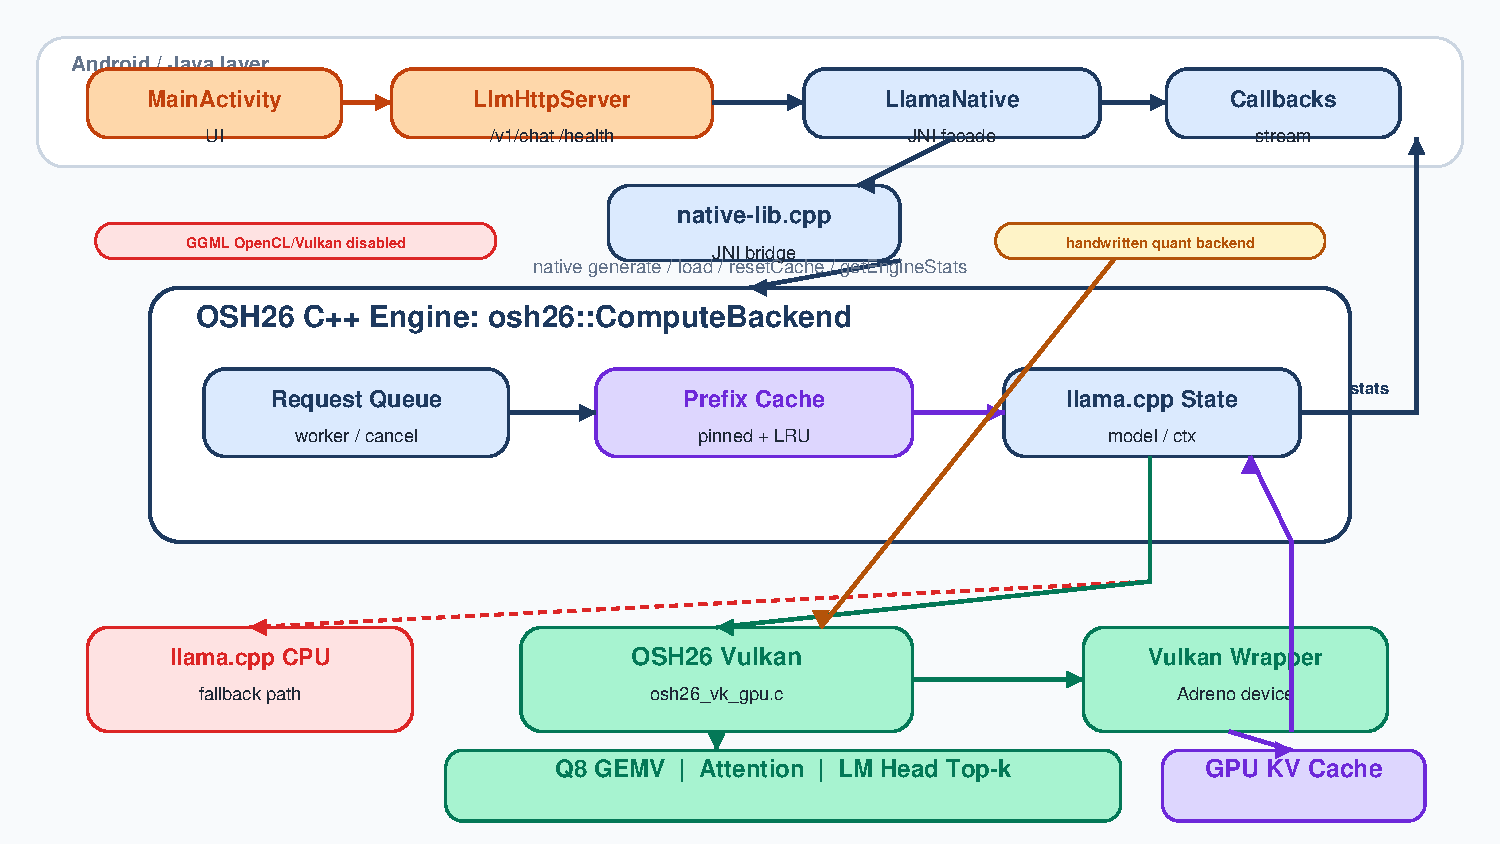
\includegraphics[width=\textwidth,height=0.84\textheight,keepaspectratio]{figures/llm-runtime-architecture.pdf}
  \end{center}
\end{frame}

\begin{frame}
  \frametitle{总体设计：CPU/GPU 分工与 KV Cache}
  \small
  移动端没有服务器级显存冗余。端侧 Runtime 需要显式管理哪些工作留在 CPU、哪些张量常驻 GPU，以及何时复用 KV。

  \vspace{0.4em}
  \scriptsize
  \begin{tabularx}{\textwidth}{p{0.20\textwidth}Y Y}
    \toprule
     & Runtime 实现 & 效果 \\
    \midrule
    控制面 / 数据面 & CPU 负责 tokenize、sampler、队列、cache policy；GPU 负责 Q8 投影、LM head、top-k & 控制逻辑保持灵活，密集计算留给 GPU \\
    工作集 & 活跃 prompt、Q8 权重、packed KV、临时 attention buffer & 避免不必要的 CPU/GPU 重复驻留 \\
    页缓存 & prefix cache page pool，按 token page 复用 K/V & 重复协议 prompt 不再完整 prefill \\
    \bottomrule
  \end{tabularx}
\end{frame}

\begin{frame}
  \frametitle{KV Cache：把上下文当虚拟内存管理}
  \begin{columns}[T,onlytextwidth]
    \begin{column}{0.48\textwidth}
      \begin{block}{Paged / Prefix 思路}
        \scriptsize
        \begin{itemize}
          \item 受 vLLM 启发：KV 不是一整块不可分割数组，而是可复用的 page。
          \item 固定系统提示词、工具协议、subagent 协议进入 pinned prefix。
          \item 普通对话使用 dynamic entry，采用LRU 回收策略。
        \end{itemize}
      \end{block}
    \end{column}
    % \begin{column}{0.48\textwidth}
    %   \scriptsize
    %   \begin{tabularx}{\textwidth}{p{0.40\textwidth}Y}
    %     \toprule
    %     指标 & 作用 \\
    %     \midrule
    %     命中状态 & 本次请求是否命中 prefix cache \\
    %     可复用 token & 可跳过 prefill 的前缀 token 数 \\
    %     Pinned entry & 固定协议前缀数量 \\
    %     碎片率 & page pool 的碎片状态 \\
    %     Restore 开销 & GPU 恢复 KV page 的时间 \\
    %     \bottomrule
    %   \end{tabularx}
    % \end{column}
  \end{columns}

  \vspace{0.35em}
  \footnotesize
  % 课程知识对应：KV Cache 类似页缓存；prefix key 类似页表索引；pinned entry 类似共享只读段；LRU / fragmentation / restore cost 决定长期运行稳定性。
\end{frame}

\begin{frame}
  \frametitle{Agent 专用优化：stateless subagent 的 pinned prefix}
  \small
  Action Fabric 会产生大量短生命周期 subagent：它们共享工具协议，但不应该继承完整聊天历史。我们把这个 workload 单独建模，而不是让它混在普通 chat cache 里。

  \vspace{0.35em}
  \scriptsize
  \begin{tabularx}{\textwidth}{p{0.24\textwidth}Y Y}
    \toprule
    场景 & 普通处理 & 我们处理 \\
    \midrule
    固定工具协议 & 每个 subagent 重新 prefill & \code{stateless\_subagent=true}，协议 prompt 进入 pinned prefix \\
    并发短任务 & 多份重复系统提示词挤占 KV & 一个 pinned entry 被多轮不同任务复用 \\
    普通聊天 & 可能和 subagent cache 混淆 & chat cache key 与 subagent cache key 分离 \\
    \bottomrule
  \end{tabularx}

  \vspace{0.55em}
  \scriptsize
  \begin{tabularx}{\textwidth}{p{0.26\textwidth}p{0.18\textwidth}p{0.18\textwidth}Y}
    \toprule
    模型 & Cold TTFT & Warm TTFT & 结论 \\
    \midrule
    0.6B-Q8\_0 & 1249.13 ms & 278.543 ms & TTFT 降低 77.7\% \\
    1.7B-Q8\_0 & 2787.45 ms & 610.29 ms & TTFT 降低 78.1\% \\
    \bottomrule
  \end{tabularx}
\end{frame}

\begin{frame}
  \frametitle{请求调度：模型服务也需要 OS 调度器}
  \begin{columns}[T,onlytextwidth]
    \begin{column}{0.52\textwidth}
      \small
      当前引擎提供 OpenAI-compatible HTTP 接口，但内部不是同步函数调用，而是带状态的 native request queue。

      \vspace{0.35em}
      \begin{itemize}
        \item \code{active\_request} 与 pending queue 分离。
        \item cancel/release 可作用于 active 与 queued request。
        \item \code{max\_pending\_requests} 提供背压。
        \item \code{prefix-aware-aging-v2} 兼顾 cache hit 与防饥饿。
      \end{itemize}
    \end{column}
    \begin{column}{0.44\textwidth}
      \scriptsize
      \begin{tabularx}{\textwidth}{p{0.38\textwidth}Y}
        \toprule
        理论 & 对应实现 \\
        \midrule
        短作业优先 & prefix hit 请求服务时间更短 \\
        Aging & cache miss 请求不会长期等待 \\
        临界区 & request state 使用锁与条件变量保护 \\
        背压 & pending queue 限制避免 UI/服务被拖垮 \\
        \bottomrule
      \end{tabularx}
    \end{column}
  \end{columns}
\end{frame}

\begin{frame}
  \frametitle{量化后端：面向 Adreno 的 Q8 数据通路}
  \scriptsize
  \begin{tabularx}{\textwidth}{p{0.23\textwidth}Y Y}
    \toprule
    模块 & 做法 & 实机意义 \\
    \midrule
    Q8\_0 权重常驻 & 使用 GGUF 原生 Q8\_0 tensor，减少重复展开与复制 & 给 8K context 和 1.7B 模型留下内存空间 \\
    W8A8 prefill & activation 动态 Q8，packed int8 dot，F32 accumulate & TTFT 主路径从 F16 prefill 7361.61 ms 降到 788.56 ms \\
    decode Q8 GEMV & \code{nt == 1} 走 subgroup \code{GEMV\_Q8} & 0.6B TPS +20.3\%，1.7B TPS +37.3\% \\
    GPU LM head & dot/top-k/merge 在 GPU 完成，只回传候选集 & 避免全词表 logits 搬回 CPU \\
    descriptor cache & 热路径 descriptor alloc 归零作为 gate & 防止系统调用开销吞掉 kernel 收益 \\
    \bottomrule
  \end{tabularx}

  \vspace{0.45em}
  \normalsize
  % 这不是“把 F32 kernel 换成 Q8 kernel”，而是把数据布局、驻留策略、候选集返回、submit/descriptor 成本和正确性 gate 一起重排。
\end{frame}

\begin{frame}
  \frametitle{优化路线：从能跑到可部署}
  \scriptsize
  \begin{tabularx}{\textwidth}{p{0.20\textwidth}Y Y}
    \toprule
    阶段 & git 历史中的工作 & 解决的问题 \\
    \midrule
    Android 闭环 & Android Studio、CPU 推理、OpenAI API、\code{configureBackend} & App 能调用模型服务 \\
    驱动探索 & 原生 Vulkan 加载成功但乱码；MNN Vulkan 基础设施；自研 compute shader & 证明原生路径不可控，转向可控后端 \\
    KV / prefill & 加 KV cache、LRU 管理、prefill 分块、GPU prefill、LM head 优化 & 降低 TTFT 与重复 prompt 成本 \\
    Q8 化 & 原生 Q8\_0、decode Q8、Q8\_0 单份权重驻留 & 降低内存与 decode latency \\
    扩展性 & 8K context、Qwen3-1.7B、消除 CPU 重复驻留 & 从 demo 模型走向可用端侧模型 \\
    Agent 化 & stateless subagent cache 策略 & 针对 Action Fabric 的真实 workload 优化 \\
    \bottomrule
  \end{tabularx}
\end{frame}

\begin{frame}
  \frametitle{实机性能与验证 gate}

  \small
  我们在红米K40真机（Adreno 650，12GB RAM）上跑Qwen3系列 0.6B-Q8\_0 和 1.7B-Q8\_0 模型，使用真实的Agent prompt序列，测量平均 TTFT、TPS
  \scriptsize
  \begin{tabularx}{\textwidth}{p{0.23\textwidth}p{0.18\textwidth}p{0.18\textwidth}Y}
    \toprule
    指标 & 0.6B-Q8\_0 & 1.7B-Q8\_0 & 说明 \\
    \midrule
    原有 TTFT median & 1249.13 ms & 2787.45 ms &  \\
    最新 TTFT median & 278.543 ms & 610.29 ms & decode Q8 GEMV 默认路径，分别提升 77.7\% 和 78.1\% \\
    原有 TPS median & 3.6718 & 1.9954 &  \\
    最新 TPS median & 6.8382 & 4.0614 & 相比旧 baseline，decode 速度分别提升 85.4\% 和 103.3\% \\
    % LM head median & 118.45 ms & 214.37 ms & GPU LM head + top-k candidate path \\
    % forward submits & 2 & 2 & 非 debug 正常路径，submit 成本受控 \\
    % descriptor alloc & 0 & 0 & 热路径 descriptor allocation 消除 \\
    % 8K context & \multicolumn{2}{c}{5488 user tokens / 43 chunks / valid output} & 证明不是只把 context 数字改大 \\
    \bottomrule
  \end{tabularx}

  \vspace{0.4em}
  \footnotesize
  % gate 不只看速度：还检查 token IDs reproducibility、logits sanity、attention fallback、top-k overlap、active request 泄漏和 debug correctness 隔离。
\end{frame}

\begin{frame}
  \frametitle{与 Action Fabric 合流：端侧 Agent OS}
  \small
  上层 Action Fabric 把 Agent 执行变成可校验、可调度、可恢复的 DAG；下层 OSH26 LLM Runtime 把本地模型变成可调度、可复用、可观测的系统服务。

  \vspace{0.4em}
  \scriptsize
  \begin{tabularx}{\textwidth}{p{0.24\textwidth}Y}
    \toprule
    Action Fabric 需求 & LLM Runtime 支撑 \\
    \midrule
    一次规划 Workflow & 本地低 TTFT 模型服务，减少云端依赖 \\
    大量短 subagent & stateless prompt + pinned prefix cache \\
    ready set 并发 & native queue、背压、prefix-aware aging \\
    失败恢复 & cancel、release、last error、token IDs、health telemetry \\
    上下文治理 & 普通 chat 与 subagent cache 隔离，避免上下文污染 \\
    \bottomrule
  \end{tabularx}

  \vspace{0.45em}
  \normalsize
  最终贡献：一个把模型、内存、驱动、调度、Action 执行统一起来的端侧 Agent Runtime。
\end{frame}


\section{项目总结}

\begin{frame}
  \frametitle{项目总结}
  \scriptsize
  本项目面向 Android 端侧智能体，构建本地部署、结构化执行、可观测、可扩展的 Agent Runtime，由端侧 LLM 推理框架与 Action Fabric 协同组成。

  \vspace{0.45em}
  \begin{block}{端侧 LLM 推理框架}
    \scriptsize
    基于 llama.cpp 与 GGUF 生态，重写适配 Adreno GPU 的 Vulkan 后端，支持 Qwen3 等小模型本地运行，并通过 Vulkan GPU 加速、Paged KV Cache、针对性 Prefix Cache 与 Q8\_0 量化，降低推理延迟、内存占用和功耗，较现有端侧框架更适合高并发、上下文格式固定的 Agent 场景。
  \end{block}

  \begin{block}{Action Fabric}
    \scriptsize
    将模型生成的任务计划结构化为有向无环图，由 Rust 调度内核完成依赖校验、Ready Set 并发调度、策略控制、失败恢复、状态存储与审计，并通过 gRPC 调用 Kotlin 侧 59 个结构化 Action。
  \end{block}

  \vspace{0.3em}
  相比传统 Agent Loop，该方案减少模型往返，降低延迟与上下文成本；相比零散工具调用，具备类型化输入输出、可信 metadata、确认门控、风险等级、副作用约束、可复现回放和工程化测试能力；相比 heavy subagent，可用更轻量的 Action 节点完成任务分解。
\end{frame}

\begin{frame}
  \frametitle{项目成员}
  \scriptsize
  \begin{tabularx}{\textwidth}{p{0.34\textwidth}p{0.22\textwidth}Y}
    \toprule
    方向 & 成员 & GitHub \\
    \midrule
    Action Fabric & 张贺淇 (负责人) & \code{@zhangheqi} \\
    & 杨家越 & \code{@jryyangjy} \\
    & 贺秋实 & \code{@SurgeHe} \\
    端侧 LLM 部署与优化 & 陈雨桥 (负责人) & \code{@SiriusPaul} \\
    & 周子墨 & \code{@alizhouzimo} \\
    \bottomrule
  \end{tabularx}
\end{frame}

\begin{frame}
  \frametitle{致谢}
  \centerline{\Large 谢谢!}
\end{frame}

\end{document}
